\documentclass[a4paper,11pt]{article}
\usepackage{jheppub} % for details on the use of the package, please see the JINST-author-manual
\usepackage{lineno}
\linenumbers
\usepackage{booktabs}
\usepackage{placeins}
\usepackage{float}
%\smartqed  % flush right qed marks, e.g. at end of proof
%
%\RequirePackage{graphicx}
%
% \RequirePackage{mathptmx}      % use Times fonts if available on your TeX system
%
% insert here the call for the packages your document requires
%\RequirePackage{latexsym}
%\RequirePackage[numbers,sort&compress]{natbib}
%\RequirePackage[colorlinks,citecolor=blue,urlcolor=blue,linkcolor=blue]{hyperref}
% etc.
%
% please place your own definitions here and don't use \def but
% \newcommand{}{}
%
%\journalname{Eur. Phys. J. C}
%

\usepackage{graphicx}
\usepackage{lineno}
\usepackage{xspace}
\linenumbers

\usepackage{color}
\definecolor{orange}{rgb}{1,0.5,0}
\definecolor{darkgreen}{rgb}{0.0, 0.6, 0.22}

\usepackage{hyperref}
\usepackage{amsmath}

\title{Balancing heavy flavor: Quantum number compensation in hadronisation of charm and beauty particles in proton–proton collisions%\thanksref{t1}
}

\author[a]{I.~Pardo Zambrana}
\emailAdd{i.pardo@student.maastrichtuniversity.nl}
\author[c]{P.~Veen}
\emailAdd{Paul.Veen@cern.ch}
\author[a,b]{K.~Vos}
\emailAdd{k.vos@maastrichtuniversity.nl}
\author[a,b]{P.~Christakoglou}
\emailAdd{Panos.Christakoglou@maastrichtuniversity.nl}

\affiliation[a]{Universiteit Maastricht,
Maastricht, The Netherlands}

\affiliation[b]{Nikhef,
Amsterdam, The Netherlands}

\affiliation[c]{Paris-Saclay IRFU CEA,
Gif-Sur-Yvette, France}



\abstract{The hadronisation of heavy quarks remains one of the least understood processes of Quantum Chromodynamics (QCD). While the production of heavy quark pairs can be calculated perturbatively in QCD, the subsequent formation of hadrons involves non-perturbative processes. These processes are predominantly model dependent and sensitive to the underlying mechanisms of colour reconnection and string fragmentation. In particular, the conservation of flavour, baryon number and charge imposes constraints on how heavy-flavour hadrons are formed and balanced within the final state.

This article presents the results from the analysis of data produced using the Pythia event generator, focusing on the investigation of how quantum numbers associated with charm and beauty production are balance in proton–proton collisions. Starting from perturbatively produced ($c\overline{c}$) and ($b\overline{b}$) pairs, we study how the formation of heavy-flavour mesons and baryons, including $D^0$, $B^+$, $\Lambda_c$, and $\Lambda_b$, is accompanied by compensating particles elsewhere in the event. The analysis focuses on correlations between the identified heavy hadron and the hadronic system responsible for balancing its conserved quantum numbers. Several hadronisation scenarios implemented in Pythia are compared, including the Monash tune, colour-reconnection models incorporating string junctions, and close-packing approaches. 

This study establishes a framework for characterising quantum-number compensation in heavy-flavour production and opens a novel avenue for testing hadronisation dynamics using identified charm- and beauty-hadron correlations.}



\begin{document}
\maketitle
\flushbottom



%________________________________________________%
%________________________________________________%
\section{Introduction}
\label{Sec:Introduction}


%\begin{figure}
%    \centering
%    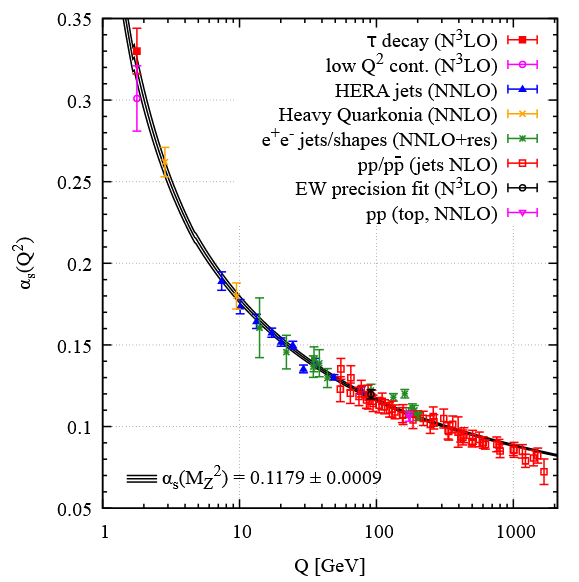
\includegraphics[width=0.5\linewidth]{figures/Introduction-figures/runningCouplingQCD.png}
%    \caption{Summary of measurements of the strong coupling constant $\alpha_{s}$ as a function of the energy scale $Q$. The relative degree of perturbation theory is shown in brackets (NLO: next-to-leading order, NNLO: next-to-next-to-leading order, N$^{3}$LO: next-to-NNLO, NNLO+res: NNLO matched to a resumed calculation). It is evident that the coupling diverges at low energies and perturbation theory starts to break down \cite{PDG} (but text literal from MSc thesis)}
%    \label{fig:secIntro:runningCouplingQCD}
%\end{figure}

The transition from coloured quarks and gluons to colour-neutral, color-singlet hadronic states, commonly referred to as hadronisation, remains one of the central open questions in Quantum Chromodynamics (QCD)~\cite{Andersson:1983ia,Webber:1994zd,Collins:1989gx,Metz:2016swz}. While the production of energetic partons can be described using perturbative techniques, the subsequent confinement of these partons into observable hadrons occurs at energy scales where the strong coupling becomes large and perturbative calculations are no longer applicable. As a result, hadronisation is usually described through phenomenological models that incorporate the essential principles of QCD while relying on experimentally constrained parameters.

The most widely used framework for describing hadronisation in high-energy collisions is the Lund string model~\cite{Andersson:1997xwk,Andersson:2002ap}. In this picture, the colour field between separating colour charges is represented by a string with approximately constant tension. As partons move apart, potential energy is stored in the string until it becomes energetically favourable to produce new quark--antiquark pairs from the vacuum. This consequently fragments the string into smaller pieces that subsequently form hadrons. Implemented in the event generator PYTHIA~\cite{Sjostrand:2014zea}, the Lund string model has been remarkably successful in describing a wide range of observables in lepton and hadron collisions.

The environment of proton--proton collisions, however, introduces additional complexity compared to the simple fragmentation of a single colour-singlet system. Multiple parton interactions (MPI), beam remnants, and overlapping colour fields generate a dense environment of colour fields. To account for these effects, PYTHIA incorporates colour reconnection (CR) mechanisms that allow partons originating from different partonic scatterings to reorganise their colour topology before hadronisation. In the Monash tune, reconnections are performed so as to minimise the overall string length, leading to an improved description of global event properties~\cite{Bierlich:2015rha}. Despite its success, the default string fragmentation framework, even with the inclusion of colour reconnections schemes encounters significant challenges when confronted with measurements of identified-particle production at the Large Hadron Collider (LHC). In particular, the observed enhancement of strange-hadron and baryon production with increasing event activity cannot be fully reproduced by conventional string fragmentation and colour reconnection models~\cite{ALICE:2016fzo}. This has motivated the development of extensions that incorporate additional non-perturbative dynamics.

One such extension is the Beyond-Leading-Colour colour reconnection model~\cite{Christiansen:2015yqa}, which introduces junction topologies. Junctions correspond to Y-shaped colour structures in which three string pieces meet at a common point, providing a natural mechanism for baryon production beyond the traditional diquark picture. The presence of junctions modifies not only baryon yields but also the correlations and balancing of conserved quantum numbers throughout the event. Another extension is the Rope Hadronisation model~\cite{Bierlich:2015rha}, in which overlapping strings combine into colour ropes with an enhanced effective string tension. The larger tension reduces the suppression of, particularly, strange quark and diquark production, leading to increased yields of strange mesons and baryons. More recently, close-packing approaches have been developed to provide a geometrically inspired description of overlapping colour fields and their collective hadronisation.

The importance of these mechanisms has been highlighted by a series of measurements performed at the LHC. In particular, the observation by the ALICE Collaboration of a strong multiplicity-dependent enhancement of strange and multi-strange hadron production in proton--proton collisions~\cite{ALICE:2016fzo} demonstrated that phenomena traditionally associated with larger collision systems are already present in small systems. Similar trends have been observed for baryon-to-meson ratios, indicating that hadron production depends not only on the flavour content of the produced quarks but also on the details of the hadronisation mechanism. Furthermore, ALICE measurements of inclusive $J/\Psi$ production as a function of charged-particle multiplicity revealed a significantly stronger-than-linear increase of the charmonium yield with event activity~\cite{ALICE:2012pet,ALICE:2021zkd}. This observation points to an important role of multiple parton interactions and suggests a non-trivial connection between heavy-flavour production and the global properties of the event. Together, these measurements have established identified-particle production, spanning both light- and heavy-flavour sectors, as a sensitive probe of non-perturbative QCD dynamics and the mechanisms governing hadron formation.

Most studies up to now have focused on light-flavour hadrons, where both the production mechanism and the hadronisation process contribute to the observed final-state particle yields. This complicates the interpretation of baryon-to-meson ratios and quantum-number correlations, since the underlying partonic production rates are themselves difficult to constrain experimentally. Heavy flavour, however, offers a unique opportunity in this respect. Charm and beauty quarks are predominantly produced in hard partonic scatterings at energy scales where perturbative QCD is applicable, and their production cross sections can, in principle, be calculated from first principles. Consequently, heavy-flavour hadrons provide a cleaner laboratory for isolating hadronisation effects from dynamics associated to partonic production.

In this work, we investigate how conserved quantum numbers are balanced during the hadronisation of heavy quarks in proton--proton collisions at LHC energies. Using PYTHIA, we compare the expectations of the Monash tune, junction-based colour reconnection, and close-packing hadronisation models. Starting from produced $c\bar{c}$ and $b\bar{b}$ pairs, we study how the formation of heavy-flavour mesons and baryons is accompanied by balancing particles elsewhere in the event using a two-particle correlations technique described in Section~\ref{Sec:Observables}. The tunes of PYTHIA and the relevant parameters used for ther production of the data samples are described in Section~\ref{Sec:Model}. The results, presented in Section~\ref{Sec:Results}, examine the flavour, baryon-number, and charge correlations associated with identified charm- and beauty-hadron production. They aim to provide new insight into the microscopic mechanisms governing hadronisation and to identify observables capable of discriminating between competing models of non-perturbative QCD.
\section{Two-particle correlations and quantum-number balancing}
\label{Sec:Observables}

Traditionally, hadronisation models are constrained through measurements of identified-particle yields and yield ratios. Examples include baryon-to-meson ratios such as $\Lambda/K^0_S$, $\Lambda_c/D^0$, or $\Lambda_b/B^+$, and measurements of strangeness enhancement as a function of event multiplicity. Such observables have proven highly valuable for identifying deficiencies in hadronisation models and motivating the development of new mechanisms such as colour reconnection, junction formation, and rope or close-packing effects. However, yield measurements provide only integrated information on the final state and are therefore often not suitable to identify the microscopic origin of the observed particles. Different hadronisation mechanisms may lead to similar integrated yields while producing very different correlation patterns among the particles generated in the same event.

Two-particle correlation techniques provide a more differential probe of hadronisation dynamics. Rather than measuring only the probability of producing a given hadron species, one studies the conditional probability of producing a second particle in the presence of a selected trigger particle. The distribution of associated particles can be investigated as a function of kinematic variables such as relative azimuthal angle $\Delta\varphi$ or pseudorapidity $\Delta\eta$. Since conservation laws operate on an event-by-event basis, the balancing partners of a given particle contain direct information about the mechanisms responsible for its production.

A particularly powerful application of this technique is the study of conserved quantum numbers. Electric charge, baryon number, strangeness, charm and beauty must be conserved globally in every collision event. Consequently, the production of a particle carrying a non-zero quantum number requires the existence of one or more balancing particles elsewhere in the event. The simplest example is electric charge conservation. If a positively charged trigger particle is selected, one may construct correlation functions with positively and negatively charged associated particles. The unlike-sign correlation function contains contributions from both charge-conserving processes and background sources unrelated to charge conservation. To isolate the balancing contribution, it is common to construct a charge-balance observable of the form

\begin{equation}
B_{\rm charge}(\Delta\eta,\Delta\varphi) = 
C_{+-}(\Delta\eta,\Delta\varphi)-
C_{++}(\Delta\eta,\Delta\varphi),
\end{equation}

\noindent where $C_{+-}$ and $C_{++}$ denote the unlike-sign and like-sign correlation functions, respectively. Equivalent definitions can be constructed using negatively charged trigger particles or by averaging positive and negative trigger samples. This subtraction removes a large fraction of the combinatorial background and highlights the particles responsible for balancing the trigger charge. The amplitude, width and shape of the resulting distribution provide information on the dynamics of local charge conservation during hadronisation. The same concept can be extended to other conserved quantum numbers. For strangeness, one may investigate correlations between strange hadrons and anti-strange hadrons. For baryon number, correlations between baryons and anti-baryons reveal how baryon-number conservation is implemented during fragmentation. Such measurements have already been proposed as sensitive probes of junction topologies, since baryons produced through junction formation are expected to exhibit balancing patterns that differ substantially from those generated through the traditional diquark mechanism.

Heavy flavour, on the other hand, offers an advantageous feature for these studies since charm and beauty quarks are produced predominantly in hard partonic scatterings as $c\bar{c}$ and $b\bar{b}$ pairs. The production process therefore establishes a well-defined heavy-flavour quantum number at the partonic level before hadronisation takes place. During fragmentation, these heavy quarks are confined into charm- and beauty-hadron species whose quantum numbers must ultimately be balanced elsewhere in the event. For example, the production of a $D^0$ meson containing a charm quark requires the corresponding anti-charm quantum number to be carried by another hadron. Similarly, the formation of a $\Lambda_c^+$ baryon involves not only charm conservation but also the redistribution of baryon number among the remaining hadrons produced during fragmentation.

The nature of these balancing partners is expected to depend strongly on the hadronisation model. In conventional string fragmentation, quantum-number compensation tends to occur locally along the fragmenting string. Junction topologies may redistribute baryon number over larger regions of phase space and alter the flavour composition of balancing particles. Likewise, close-packing mechanisms may modify the probabilities for producing heavy quarks and diquarks, potentially changing both the species and kinematic distributions of the balancing hadrons. Consequently, two-particle correlation measurements provide information that is largely inaccessible through inclusive yield measurements alone.

In the present work, we extend the concept of quantum-number balancing to the heavy-flavour sector. By selecting identified charm and beauty mesons and baryons as trigger particles and studying their correlations with associated heavy-flavour particles, we investigate how charm, beauty, charge, and baryon number are compensated in different PYTHIA hadronisation models. The resulting correlation patterns provide a direct probe of the microscopic mechanisms governing heavy-flavour hadronisation.
\FloatBarrier
\section{Data samples}
\label{Sec:Model}
%PYTHIA
%- Overview of PYTHIA
%- How is hadronisation described in PYTHIA
%- Tunes
%    - MONASH
%    - JUNCTIONS
%    (we could also look at:
%    - Close-packing
%    - Ropes)
%Table with number of events, number of generated b and c quarks, yield of B+, B-, $\Lambda_b$ (and bar), D+, D-, $\Lambda_c$ (and bar).
%Multiplicity spectra
%Some kinematic spectra (pT, $\eta$, $\phi$, etc.) for the particles we care about. We can move this to some appendix but it will be nice to have here as an overview.


This section describes the simulated pp samples used in the analysis, the common particle-level selections, and the three PYTHIA~8 hadronisation configurations compared throughout the paper: MONASH, JUNCTIONS, and CLOSEPACKING.

\subsection{PYTHIA~8 setup}
\label{sec:pythia-setup}

Events are generated with PYTHIA~8 using the Lund string model for hadronisation.  Proton--proton collisions are generated at $\sqrt{s} = 14~\mathrm{TeV}$. The samples are hard-heavy-flavour enriched samples rather than minimum-bias samples.  
The common generator settings are summarized in Table~\ref{tab:generator-settings}.

\begin{table}[tbp]
\centering
\label{tab:generator-settings}
\begin{tabular}{ll}
\toprule
Setting & Value \\
\midrule
Collision system & pp \\
Centre-of-mass energy & $\sqrt{s}=14~\mathrm{TeV}$ \\
Beam IDs & \texttt{Beams:idA = 2212}, \texttt{Beams:idB = 2212} \\
Baseline tune & \texttt{Tune:pp = 14} \\
Hard charm production & \texttt{HardQCD:hardccbar = on} \\
Hard beauty production & \texttt{HardQCD:hardbbbar = on} \\
Hard-process cut & \texttt{PhaseSpace:pTHatMin = 1.} \\
Events per job & $10^{6}$ \\
Jobs per tune & $100$ \\
Events per tune & $10^{8}$ \\
\bottomrule
\end{tabular}
\caption{Common PYTHIA~8 generator settings used for all three hadronisation configurations.}
\end{table}

\subsection{Particle selection}
\label{sec:particle-selection}

Particles are selected at generator level after hadronisation.  The analysis uses final-state particles satisfying $p_{\mathrm{T}} \geq 0.15~\mathrm{GeV}/c$ and $|\eta| \leq 4$. The weakly decaying heavy-flavour hadrons used in the analysis are kept stable at generator level by disabling their decays.

The charged-particle multiplicity, $N_{\mathrm{ch}}$, is defined using prompt charged particles in the same kinematic acceptance with PYTHIA status codes in the prompt range used by the analysis.

\subsection{Hadronisation models}
\label{sec:hadronisation-models}

The same hard-process setup and particle-level selections are used for all three configurations.  The configurations differ only in the modelling of hadronisation, colour reconnection, and dense-string effects.

\subsubsection{MONASH}
\label{sec:monash}

The MONASH configuration is used as the baseline PYTHIA~8 reference tune.  It corresponds to the Monash 2013 tune, which provides a global tuning of fragmentation, multiparton interactions, colour reconnection, and underlying-event parameters.

This configuration is used as the reference because it is the standard PYTHIA~8 pp tune and provides the baseline expectation for heavy-flavour hadronisation without the additional junction or close-packing mechanisms studied here.

\subsubsection{JUNCTIONS}
\label{sec:junctions}

The JUNCTIONS configuration uses the QCD-based colour-reconnection model with junction topologies enabled.  In this model, colour reconnections are guided by QCD colour rules and by minimization of the string-length measure. 

\subsubsection{CLOSEPACKING}
\label{sec:closepacking}

The CLOSEPACKING configuration includes the string close-packing model.  The model accounts for the effect of overlapping strings in high-density pp events.  Close strings modify the effective string tension, which can affect strangeness production, transverse-momentum spectra, and baryon production.

\subsection{Generated samples}
\label{sec:generated-samples}

For each configuration, $100$ independent jobs are generated, each containing $10^{6}$ events.  The total generated sample therefore contains $10^{8}$ events per configuration and $3\times10^{8}$ events overall.  The generated sample sizes and selected heavy-flavour hadron yields are shown in Table~\ref{tab:generated-heavy-flavour-summary}.

\begin{table}[tbp]
\centering
\label{tab:generated-heavy-flavour-summary}
\begin{tabular}{lrrrr}
\toprule
Observable & MONASH & JUNCTIONS & CLOSEPACKING & Overall \\
\midrule
$N_{\mathrm{ev}}$ & $100\,000\,000$ & $100\,000\,000$ & $100\,000\,000$ & $300\,000\,000$ \\
$N_{b+\bar b}^{\mathrm{acc}}$ & $13\,321\,922$ & $13\,258\,188$ & $13\,263\,640$ & $39\,843\,750$ \\
$N_{c+\bar c}^{\mathrm{acc}}$ & $125\,387\,414$ & $124\,842\,736$ & $125\,437\,031$ & $375\,667\,181$ \\
\midrule
$B^{+}$ & $2\,853\,111$ & $2\,044\,989$ & $2\,004\,038$ & $6\,902\,138$ \\
$B^{-}$ & $2\,841\,524$ & $2\,036\,333$ & $2\,004\,631$ & $6\,882\,488$ \\
$\Lambda_{b}^{0}$ & $219\,087$ & $472\,196$ & $973\,428$ & $1\,664\,711$ \\
$\overline{\Lambda}_{b}^{0}$ & $208\,457$ & $474\,179$ & $982\,931$ & $1\,665\,567$ \\
$D^{+}$ & $18\,422\,929$ & $16\,436\,770$ & $16\,405\,528$ & $51\,265\,227$ \\
$D^{-}$ & $18\,474\,130$ & $16\,514\,161$ & $16\,493\,255$ & $51\,481\,546$ \\
$\Lambda_{c}^{+}$ & $2\,282\,077$ & $8\,039\,633$ & $7\,296\,136$ & $17\,617\,846$ \\
$\overline{\Lambda}_{c}^{-}$ & $2\,238\,580$ & $7\,887\,369$ & $7\,195\,995$ & $17\,321\,944$ \\
\bottomrule
\end{tabular}
\caption{Generated-event sample sizes and selected heavy-flavour hadron yields for the three PYTHIA~8 configurations.}
\end{table}

\subsection{Multiplicity classes}
\label{sec:multiplicity-classes}

Event activity classes are defined using percentiles of the charged-particle multiplicity distribution, $N_{\mathrm{ch}}$.  The classes used throughout the analysis are
\begin{equation}
0\text{--}1\%,\ 
1\text{--}10\%,\ 
10\text{--}20\%,\ 
20\text{--}30\%,\ 
30\text{--}40\%,\ 
40\text{--}50\%,\ 
50\text{--}60\%,\ 
60\text{--}70\%,\ 
70\text{--}80\%,\ 
80\text{--}90\%,\ 
90\text{--}100\%.
\end{equation}

The $0$--$1\%$ class corresponds to the highest-multiplicity events, while the $90$--$100\%$ class corresponds to the lowest-multiplicity events.

\begin{figure}[tbp]
    \centering
    
\includegraphics[width=0.85\linewidth]{figures/Kinematic Plots/MultiplicitySpectrum_Shared_shape.png}
    \caption{Charged-particle multiplicity distribution for the generated hard-heavy-flavour event samples. The charged-particle multiplicity $N_{\mathrm{ch}}$ is defined using prompt charged particles with $p_{\mathrm{T}}\geq0.15~\mathrm{GeV}/c$ and $|\eta|\leq4$ in pp collisions at $\sqrt{s}=14~\mathrm{TeV}$.}
    \label{fig:mult_distribution}
\end{figure}

\FloatBarrier
\section{Results and publication status}
\label{sec:results}

\subsection{Multiplicity-integrated balancing yields}

Table~\ref{tab:integrated} records pooled full-axis balancing yields and their
ten-block standard errors. The values are retained in a committed plotting-log
fixture. The fixture contains twelve finite-yield rows with ten finite blocks,
but it omits the pair-count rows required to reproduce the registered
integer-exact integrated closure. The numbers are therefore reportable as a
labelled validation result, not as a closed final-figure source.\claim{R1}

\begin{table}[H]
\centering
\caption{Multiplicity-integrated signed balancing yields per trigger. The
source is the retained nominal validation fixture; the original pair-count log
needed for integer-exact closure is unavailable.}
\label{tab:integrated}
\begin{tabular}{llcc}
\toprule
Sector & Tune bundle & Reference meson & Baryon \\
\midrule
Beauty & MONASH       & $B^-: 0.11625\pm0.00027$ & $\Lambda_b: 0.01942\pm0.00010$ \\
Beauty & JUNCTIONS    & $B^-: 0.08730\pm0.00035$ & $\Lambda_b: 0.03653\pm0.00031$ \\
Beauty & CLOSEPACKING & $B^-: 0.08550\pm0.00023$ & $\Lambda_b: 0.03330\pm0.00022$ \\
Charm  & MONASH       & $D^-: 0.19345\pm0.00012$ & $\bar\Lambda_c^-: 0.01893\pm0.00005$ \\
Charm  & JUNCTIONS    & $D^-: 0.17397\pm0.00013$ & $\bar\Lambda_c^-: 0.02402\pm0.00003$ \\
Charm  & CLOSEPACKING & $D^-: 0.17348\pm0.00010$ & $\bar\Lambda_c^-: 0.02076\pm0.00004$ \\
\bottomrule
\end{tabular}
\end{table}

Relative to MONASH, both non-baseline bundles have a lower integrated
reference-meson balancing yield and a higher integrated baryon balancing yield
in the beauty sector. The charm baryon shift is also positive in both bundles,
while the reference-meson yield is lower. These are comparisons between full
configuration bundles and do not identify their microscopic cause. They are
also conditioned on job completion. The recorded attempt rates are tune
dependent: 0/1,000 for MONASH, 63/1,063 for JUNCTIONS, and 64/1,064 for
CLOSEPACKING. Because the recorded hang is in
\pathcode{JunctionSplitting} and event-content independence is unmeasured,
these comparisons are not accepted publication inferences.

\subsection{Beauty baryon/reference-meson trend}

The committed class-resolved table provides the $\Lambda_b/B^-$ signed
balancing-yield ratio for all eleven common classes. Table~\ref{tab:endpoints}
shows its lowest- and highest-activity endpoints and the primary endpoint
contrast. The central contrast is formed as $R(\mathrm{c11})-R(\mathrm{c1})$;
its quoted uncertainty here is statistical only.\claim{R2}

\begin{table}[H]
\centering
\caption{Endpoint contrast of the beauty $\Lambda_b/B^-$ balancing-yield
ratio. Uncertainties in this table are ten-block statistical SEMs.}
\label{tab:endpoints}
\begin{tabular}{lccc}
\toprule
Tune bundle & $R(\mathrm{c1})$ & $R(\mathrm{c11})$ & $R(\mathrm{c11})-R(\mathrm{c1})$ \\
\midrule
MONASH       & $0.18645\pm0.00692$ & $0.16192\pm0.00258$ & $-0.02453\pm0.00739$ \\
JUNCTIONS    & $0.21408\pm0.00873$ & $0.54317\pm0.00590$ & $+0.32909\pm0.01053$ \\
CLOSEPACKING & $0.21624\pm0.00765$ & $0.50344\pm0.01129$ & $+0.28719\pm0.01364$ \\
\bottomrule
\end{tabular}
\end{table}

The non-baseline bundle contrasts exceed the MONASH contrast in the committed
central table. The stored systematic verdict gives contrast differences of
$0.35362\pm0.16134$ for JUNCTIONS minus MONASH and
$0.31172\pm0.15666$ for CLOSEPACKING minus MONASH, where the uncertainty is the
stored combined total.\claim{R3} Those totals exclude S4 and descend from the
2026-08-21 two-SEM correction. They are
included to synchronize the draft with the measured repository state, not to
license a final significance statement. No trial correction across the 72
stored comparisons or cross-class covariance estimate is available.

The paper-facing charm baryon/reference-meson quantity uses the signed
$\bar\Lambda_c^-/D^-$ registry definition. A complete machine-readable charm
matrix and an accepted P8 canvas are absent, so this draft quotes no charm
ratio trend and makes no charm-versus-beauty ratio comparison.\claim{R4}

\subsection{Blocked scientific figure programme}

The machine-readable figure manifest records eight candidate roles and zero
accepted outputs. Accordingly, this build contains no scientific figure
environment and no image copied from the historical paper tree. It also does
not use the three internal explanatory SVGs.\claim{F0}

Table~\ref{tab:figure-programme} preserves the intended paper order without
turning a planned role into a figure claim. In particular, roles P2 and P3
remain the charm and beauty correlation figures. The later balancing roles use
the current combined-canvas layout rather than the obsolete pair of separate
charm and beauty files.

\begin{table}[H]
\small
\centering
\caption{Planned publication figure roles. ``Candidate'' is the manifest
status, not acceptance. No row contributes image bytes to this manuscript
build.}
\label{tab:figure-programme}
\begin{tabularx}{\textwidth}{c l X l}
\toprule
Order & Role & Required current presentation & Status \\
\midrule
P1 & Event classification & Shared 13.6~TeV spectrum and common c1--c11 boundaries & Candidate \\
P2 & Charm correlations & Per-trigger MONASH charm OS, SS, and OS--SS angular correlations & Candidate \\
P3 & Beauty correlations & Per-trigger MONASH beauty OS, SS, and OS--SS angular correlations & Candidate \\
P4/P6 & Integrated yields & One V-INTEGRATED canvas may carry charm and beauty after an explicit packaging ruling & Candidate \\
P5/P7 & Activity-dependent yields & Combined charm and beauty canvas; V-FULL versus V-EXTREMES remains open & Candidate \\
P8 & Signed ratios & Registry-resolved $\bar\Lambda_c^-/D^-$ and $\Lambda_b/B^-$ ratios & Candidate \\
\bottomrule
\end{tabularx}
\end{table}

Acceptance requires the exact ROOT-derived output bytes at the canonical
role-specific result path, configuration and source digests, selector
authorization, central and ten-block input identities, machine-readable
points, a v1 acceptance receipt, pinned runtime, and clean visual and
scientific review. The inaccessible external products, absent final bytes,
incomplete S4 result, integrated-log gap, unbounded hang-selection risk,
unrevalidated external pair sidecars, and absent corrected rerenders remain
release blockers.\claim{F9}

\section{Summary}
\label{sec:summary}

We have synchronized a manuscript description of heavy-flavour
quantum-number balancing with the repository's current scientific contracts.
The observable is an ordered, signed, per-trigger heavy-hadron correlation,
with factor-one same-sign subtraction and a dedicated trigger count.\claim{S1}
The central event-activity axis consists of eleven common absolute classes,
and the statistical uncertainty is the standard error of the complete
estimator across ten disjoint file blocks. The operational activity predicate
is final, charged, non-heavy, $p_{\mathrm{T}}>0.15$~GeV/$c$, and
$|\eta|\leq1$; its measured 0.7670\% minimum-bias production-decay mismatch
causes no class migration under the current boundaries but is unmeasured in
the forced hard-heavy sample.\claim{S2}

The committed tables show that the full JUNCTIONS and CLOSEPACKING bundles
redistribute the beauty balancing yield from the $B^-$ reference channel
towards $\Lambda_b$ as activity increases relative to the MONASH bundle. The
stored central endpoint contrasts are positive for both non-baseline bundles
and slightly negative for MONASH.\claim{S3} This conclusion is a comparison of
complete configurations. It does not isolate colour reconnection, junctions,
close packing, or any other individual setting.

The paper is not release-ready. The class-resolved systematic budget lacks S4,
the tune-dependent generator-hang selection risk is unbounded, and the external
ROOT products and accepted P1--P8 bytes are unavailable in this checkout.
MONASH recorded 0 hangs in 1,000 attempts, while JUNCTIONS recorded 63 in
1,063 (5.93\%) and CLOSEPACKING 64 in 1,064 (6.02\%). The hang is recorded in
\pathcode{JunctionSplitting}; whether completion is independent of event
content and the published observables has not been measured.\claim{S4} The
present PDF therefore records the analysis and its
measured, explicitly qualified tables while failing closed on final figures
and release-level inference.

%------------------------------------------------%

%------------------------------------------------%
\section*{Acknowledgements}
We are grateful... 
%------------------------------------------------%

% BibTeX users please use one of
\bibliographystyle{utphys}
\bibliography{hfBalancingModelPaperRefs}{}

\end{document}

